\section{Examples}
Use the following examples when you use equations, figures and tables.

\section{Equation}
You can put inline equation with \$ like $E=mc^2$. If you use equation or align environment, you can display equations as following:
\begin{align}
    L_p^{|\ell|}(x) = \sum_{r=0}^{p}(-1)^r\mqty(p+|\ell|\\p-r)\cfrac{x^r}{r!}. \label{eq:laguerre}
\end{align}
You can refer exiting equation with labels defined in the equation like \eqref{eq:laguerre}.

Physics package is useful for complex equations. See \url{http://mirrors.ibiblio.org/CTAN/macros/latex/contrib/physics/physics.pdf} for more info.

\subsection{Figure}
You can use \textbackslash includegrahics to display figures, usually in figure environment. Example is shown in \figref{fig:einstein}.
\begin{figure}[htbp] % htbp: position controller
    \centering
    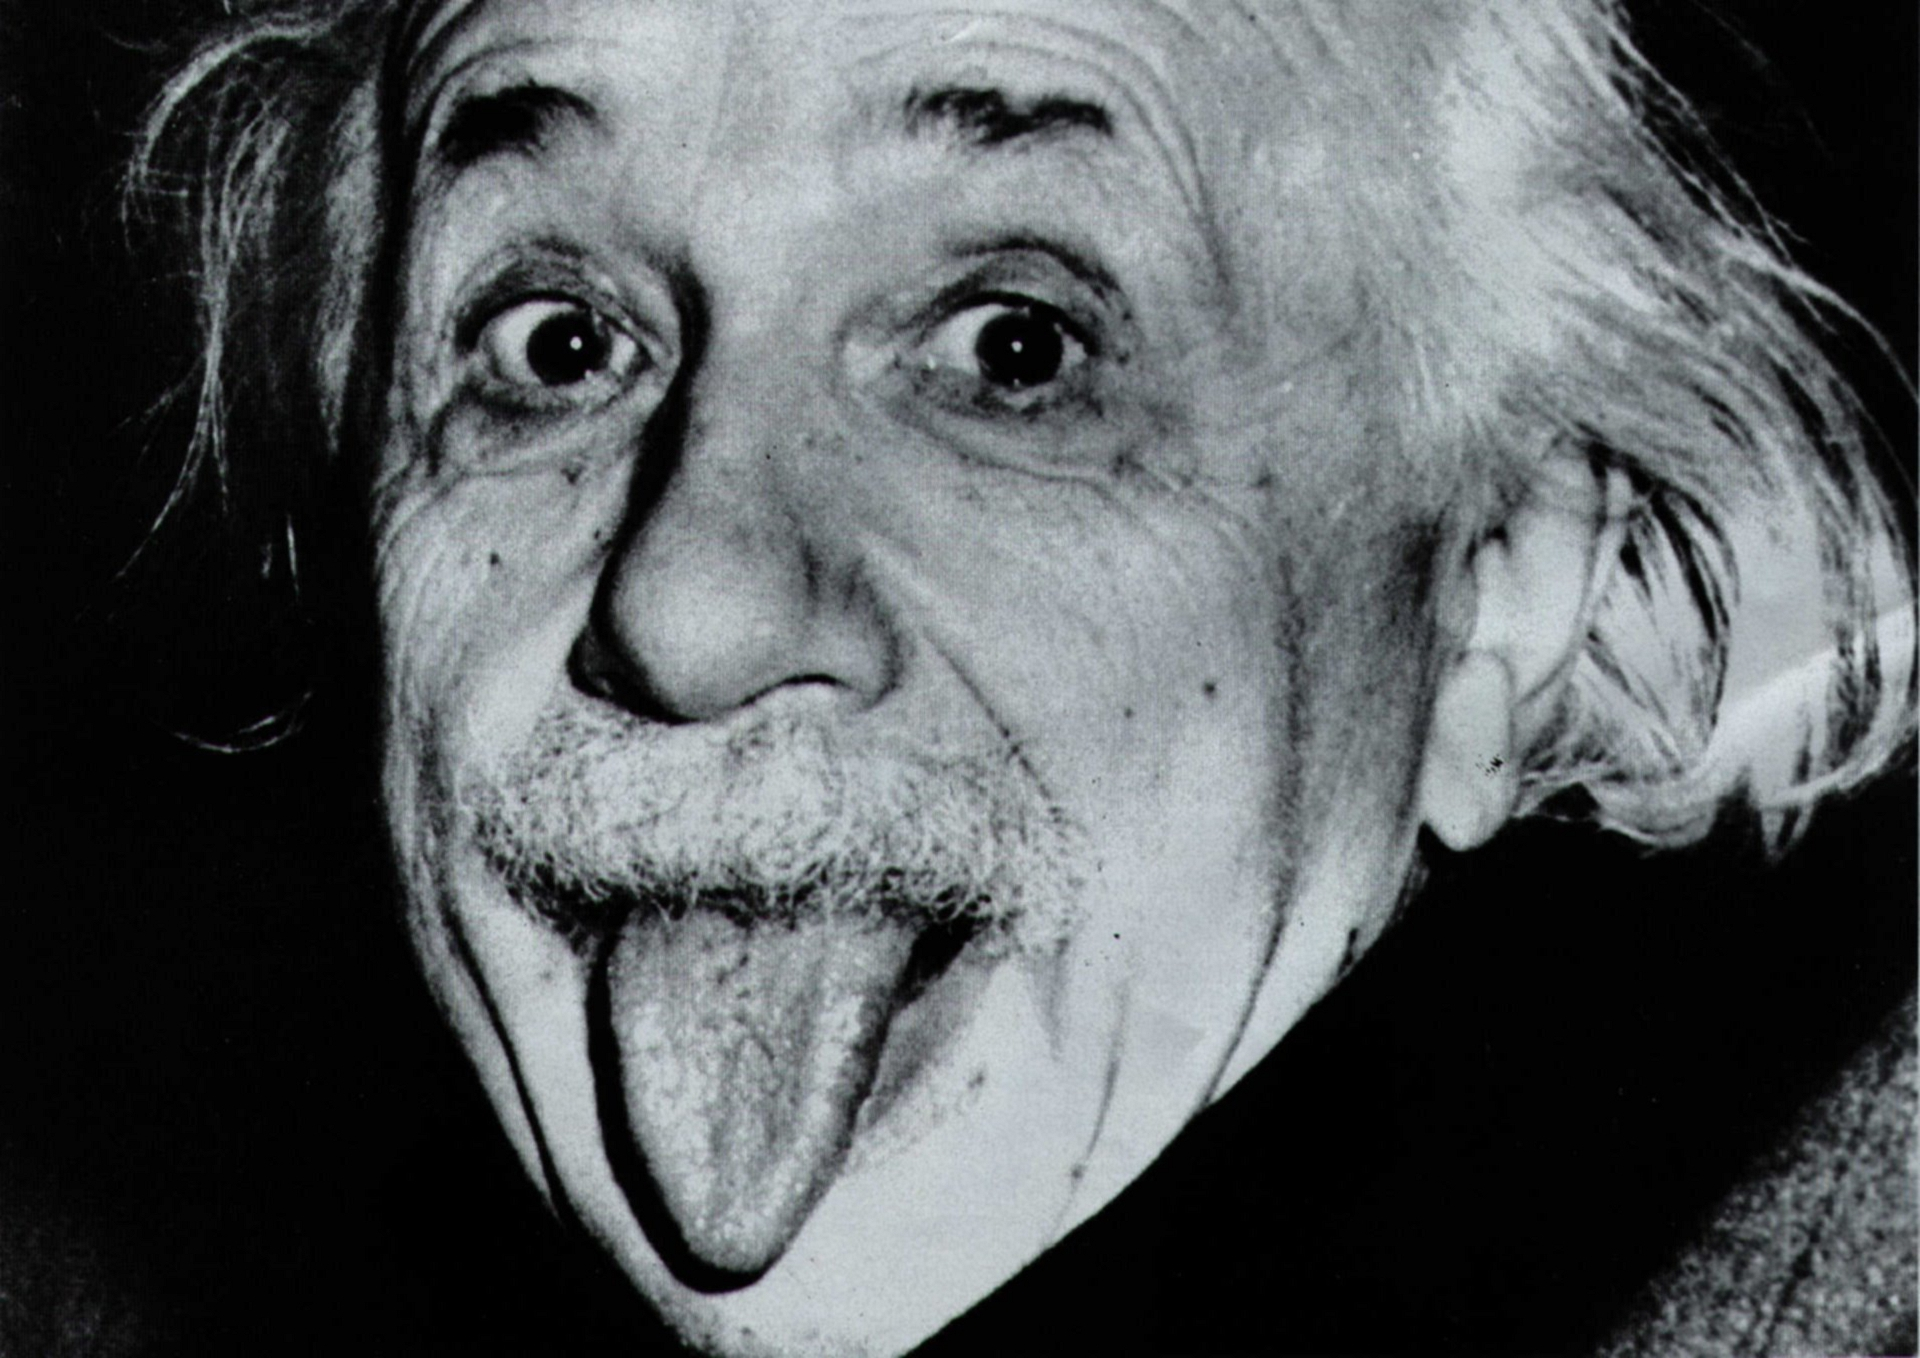
\includegraphics[width=0.9\linewidth]{Figures/Chapter2/einstein.jpeg}
    \caption{Albert Einstein}
    \label{fig:einstein}
\end{figure}

\subsection{Table}
Use table generator \url{https://www.tablesgenerator.com/} and paste it to display tables.

\subsection{Citation}
You can refer to previous works with cite command\cite{maiman1960stimulated}. The argument inside cite command can be multiple delimited by comma. The cited reference materials will be displayed in the Bibliography automatically ordered by appearance.